% $Id: serverConfigPrefPage.tex 10532 2010-03-16 15:57:20Z alexandra $
% Local Variables:
% ispell-check-comments: nil
% Local IspellDict: american
% End:
% --------------------------------------------------------
% User documentation
% copyright by BREDEX GmbH 2004
% --------------------------------------------------------

\label{TasksPrefsAgent}
\index{Preferences!AUT Agent}
\index{AUT Agent!Preferences}
\index{Add!AUT Agent}
\index{AUT Agent!Add}

You can find the \gdagent{} preference page under:\\
\bxname{Test-\gdagent{}}\\
in the preferences dialog.


\begin{enumerate}
\item In the \gdagent{} preference page, you can add, edit and delete \gdagent{}s and port numbers. 
\item The hostnames and port numbers you enter here are displayed in the drop-down list for the \bxcaption{Connect to \gdagent{}} button on the toolbar. You will be able to connect to these hostnames on these port numbers when you have started an \gdagent{} on them \bxpref{TasksAgentExternal}.
\bxtipp{The \gdagent preference page can also be accessed from the \gdaut{} configuration dialog which you can open from the \gdproject{} properties.}
\end{enumerate}


\begin{figure}[p]
\begin{center}
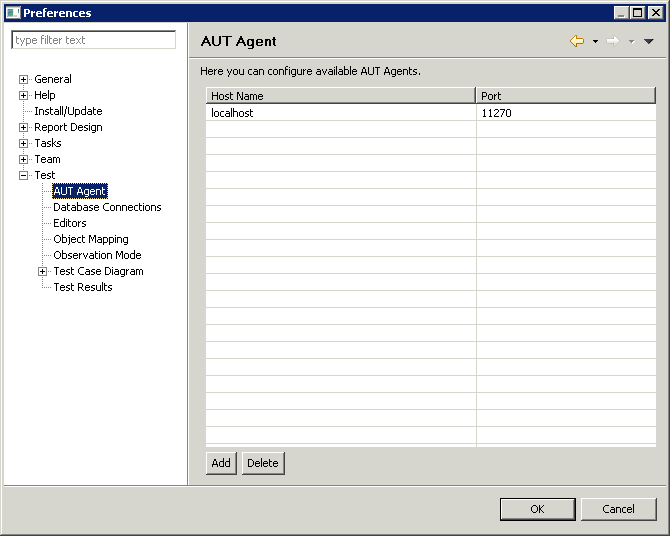
\includegraphics[width=12.5cm]{Tasks/Preferences/PS/serverconfig}
\caption{\gdagent Configuration Dialog}
\label{serverconfig}
\end{center}
\end{figure}







